\documentclass[11pt]{article}
\usepackage[margin=1in]{geometry}
\usepackage{amsmath,amssymb,amsthm,booktabs,microtype,enumitem,array,tikz}
\usepackage[colorlinks=true,linkcolor=blue!45!black,citecolor=blue!45!black,urlcolor=blue!45!black]{hyperref}
\hypersetup{pdftitle={Depegs are holes: when an on-chain coin is money},pdfauthor={William Alubokho Ashioya}}

\newtheorem{theorem}{Theorem}
\newtheorem{lemma}[theorem]{Lemma}
\newtheorem{proposition}[theorem]{Proposition}
\newtheorem{corollary}[theorem]{Corollary}
\theoremstyle{definition}
\newtheorem{definition}[theorem]{Definition}
\newtheorem*{assumption}{Assumption A}
\theoremstyle{remark}
\newtheorem{remark}[theorem]{Remark}
\newcommand{\R}{\mathbb{R}}
\newcommand{\eps}{\varepsilon}
\newcommand{\fc}[1]{\lVert #1\rVert}
\setlength{\emergencystretch}{2em}
\setlist{itemsep=2pt,topsep=4pt}

\title{Depegs are holes:\\ when an on-chain coin is money}
\author{William Alubokho Ashioya\thanks{\texttt{waa6673@nyu.edu}. The length bound used in Section~\ref{sec:leash} is joint work with Elmar Langetepe~\cite{LA}. This note was prepared with the assistance of the AI system Claude (Anthropic).}}
\date{12 November 2026}

\begin{document}
\maketitle

\begin{abstract}
A stablecoin promises that one coin is one dollar. We treat every place where the coin can be exchanged (a pool, a mint-and-redeem contract, a bank, a mobile-money ramp) as a link that carries an exchange rate, and every round trip that can be completed in one transaction as a filled cell. Arbitrage keeps each filled cell within its fees. Three statements follow. (1)~Along any route, the price of the coin differs from par by at most the fees of the cells needed to fill the loop between that route and the par link. (2)~If the par link is not a contract on the chain, the loop is a hole, and no on-chain arbitrage bounds the deviation. (3)~Coins joined by an on-chain par link carry the same deviation until the capacity of that link is used up. The Federal Reserve's account of the run on USDC in March 2023~\cite{Fed} shows all three. We then solve two design problems in closed form. Stability: redeem pro rata, hold reserve legs with weights $w_i\propto1/d_i$, and keep a first-loss buffer $b^*=1/(\sum_i 1/d_i-1)$, where $d_i$ is the largest loss of leg~$i$. Distribution: one escrowed leg per group of users, and payment sessions of at least $(g_o+g_r)/(\tau p)$ payments. What remains is the link between the reserve asset and central bank money, which only regulation can close.
\end{abstract}

\section{Model}

\emph{Assets} are dollars in a bank (USD), shillings on M-Pesa (KES), and tokens on a chain (USDC, ETH, the coin~$s$). A \emph{venue} is any place where one asset is exchanged for another: a pool, a mint-and-redeem contract, an order book, a bank, a mobile-money ramp. A venue $e$ between assets $i$ and $j$ gives $e^{m_e-f_e}$ units of $j$ for one unit of $i$, and $e^{-m_e-f_e}$ units of $i$ for one unit of~$j$. Here $m_e$ is the mid log-rate, and $f_e\ge0$ is the half-spread: the fee, plus the price impact and the gas cost per unit at the size considered. Each venue has a \emph{capacity}, the largest size it serves on these terms.

A \emph{route} is a sequence of venues, and a \emph{loop} is a route that returns to its start. For a route or loop $C$ write $m(C)$ for the sum of its mid log-rates, each taken with the sign of the direction of travel, and $f(C)$ for the sum of its half-spreads. One unit sent around a loop $C$ returns as $e^{m(C)-f(C)}$ units. A loop is \emph{atomic} if it can be executed in a single transaction, that is, if every venue on it is a contract on the same chain. We call an atomic loop a \emph{cell} (Figure~\ref{fig:complex}).

\begin{assumption}
At the end of every block, no cell returns more than was sent, in either direction.
\end{assumption}

This is the law of one price in its on-chain form. A violation is a risk-free profit that anyone can take in one transaction, and arbitrage programs take it.

\begin{lemma}\label{lem:cell}
Under Assumption~A every cell $P$ satisfies $|m(P)|\le\eps_P:=f(P)$.
\end{lemma}

\begin{proof}
Forwards the cell returns $e^{m(P)-f(P)}\le1$, and backwards $e^{-m(P)-f(P)}\le1$.
\end{proof}

We extend $m$ linearly to formal combinations of venues with real coefficients. A \emph{filling} of a loop $C$ is a combination of cells $S=\sum_Pn_PP$ whose loops add up to $C$, written $\partial S=C$. The \emph{filling cost} of $C$ is
\[
  \fc{C}=\min\Bigl\{\sum_P|n_P|\,\eps_P:\ \partial S=C\Bigr\},
\]
and $C$ is a \emph{hole} if it has no filling.

\begin{definition}\label{def:money}
The coin $s$ is \emph{money for a group of users}, with tolerance $\tau$ and size $c$, if a member can buy it at any time and sell it at any later time, in any amount up to $c$, and receive at least $e^{-\tau}$ times the dollar value paid.
\end{definition}

\begin{figure}[t]
\centering
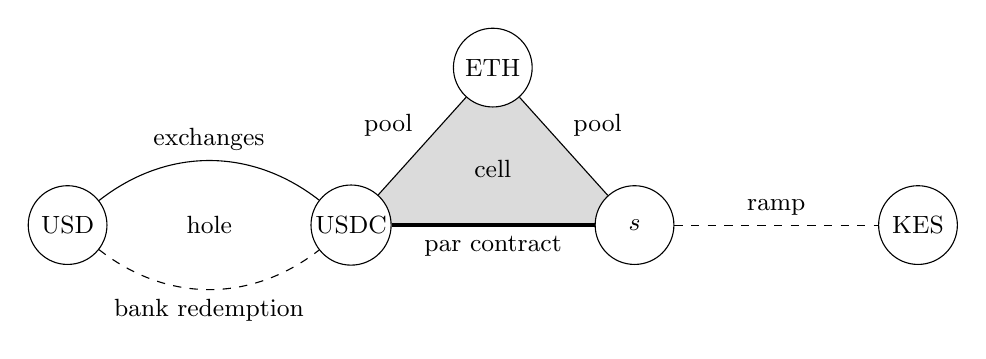
\begin{tikzpicture}[every node/.style={font=\small},asset/.style={circle,draw,fill=white,inner sep=1pt,minimum size=10mm}]
\fill[gray!28] (3.6,0)--(5.4,2.0)--(7.2,0)--cycle;
\node[asset] (usd) at (0,0) {USD};
\node[asset] (usdc) at (3.6,0) {USDC};
\node[asset] (eth) at (5.4,2.0) {ETH};
\node[asset] (s) at (7.2,0) {$s$};
\node[asset] (kes) at (10.8,0) {KES};
\draw (usdc)--(eth) node[midway,above left] {pool};
\draw (eth)--(s) node[midway,above right] {pool};
\draw[very thick] (usdc)--(s) node[midway,below] {par contract};
\draw (usd) to[bend left=38] node[midway,above] {exchanges} (usdc);
\draw[dashed] (usd) to[bend right=38] node[midway,below] {bank redemption} (usdc);
\draw[dashed] (s)--(kes) node[midway,above] {ramp};
\node at (5.4,0.72) {cell};
\node at (1.8,0) {hole};
\end{tikzpicture}
\caption{Assets, venues, a cell and a hole. Solid links are contracts or markets that trade at every hour; dashed links are off-chain and can stop. The loop of the two pools and the par contract can be executed in one transaction, so it is a cell. The loop between the market price of USDC and its redemption at a bank cannot, so it is a hole.}
\label{fig:complex}
\end{figure}

\section{Three statements about the peg}

\begin{theorem}[Filling bound]\label{thm:fill}
Assume~A. If a loop $C$ has a filling $S=\sum_Pn_PP$, then $|m(C)|\le\sum_P|n_P|\,\eps_P$. Hence $|m(C)|\le\fc{C}$.
\end{theorem}

\begin{proof}
$m(C)=m(\partial S)=\sum_Pn_P\,m(P)$, and $|m(P)|\le\eps_P$ by Lemma~\ref{lem:cell}.
\end{proof}

\begin{corollary}[Routes and the peg]\label{cor:peg}
\textup{(a)} For two routes $\gamma,\gamma'$ between the same assets, $|m(\gamma)-m(\gamma')|\le\fc{\gamma-\gamma'}$: both routes give the same price up to the filling cost of the loop between them.
\textup{(b)} Let $\pi$ be a \emph{par venue} between the coin $s$ and an asset $u$: it mints and redeems one for one, with fee $\varphi$ each way, so $m_\pi=0$ and $f_\pi=\varphi$. Then every route $\gamma$ from $s$ to $u$ satisfies $|m(\gamma)|\le\fc{\gamma-\pi}$.
\end{corollary}

For a pool between $s$ and $u$ with fee $f$, the loop $\gamma-\pi$ is itself a cell, and the deviation from par is at most $f+\varphi$. Through a third asset $x$ it is at most $f_{sx}+f_{xu}+\varphi$. With the fee tiers $0.01\%$ and $0.05\%$ that are common on Base, these are $1$ and $10$ basis points plus~$\varphi$. The bounds hold for sizes within the capacities of the venues used. For the par venue the capacity is the reserve.

\begin{theorem}[Holes]\label{thm:hole}
Let $C$ be a hole. For every real number $h$ there are mid-rates $m$ with $m(P)=0$ for every cell $P$ and $m(C)=h$.
\end{theorem}

\begin{proof}
The loops of cells span a linear subspace of the space of combinations of venues, and $C$ is not in it. So there is a linear functional that vanishes on this subspace and equals $h$ at~$C$. Its values on the venues are the~$m_e$.
\end{proof}

For a hole, Assumption~A therefore says nothing about $m(C)$. We call $m(C)$ the \emph{flux} through the hole. A loop through a venue that is not a contract on the chain (a bank, a ramp, a centralised exchange) is a hole unless other cells fill it. Only slow arbitrage limits its flux: capital, settlement time, and the risk that the off-chain venue fails. The flux can have either sign.

\begin{proposition}[Coins joined at par]\label{prop:glue}
Assume~A. Let $\pi_{st}$ be a par venue between two coins $s$ and $t$, and let $\gamma_s$, $\gamma_t$ be routes from $s$ and from $t$ to the same asset~$u$. Then
\[
  |m(\gamma_s)-m(\gamma_t)|\le\fc{\gamma_s-\gamma_t-\pi_{st}} .
\]
If both coins trade against a common asset in pools with fees $f_s$ and $f_t$, their prices differ by at most $f_s+f_t+\varphi_{st}$, whatever happens to either peg. The bound lapses when the capacity of $\pi_{st}$ is used up.
\end{proposition}

\begin{proof}
The route $\gamma_s$, then $\gamma_t$ backwards, then $\pi_{st}$ backwards is a loop with $m=m(\gamma_s)-m(\gamma_t)$. Apply Theorem~\ref{thm:fill}. Without $\pi_{st}$ the cells that contain it are not available.
\end{proof}

\subsection*{March 2023}

On 10 March 2023 Silicon Valley Bank failed. Circle disclosed that $\$3.3$ billion of about $\$40$ billion of USDC reserves was held there, $8.25\%$. Table~\ref{tab:svb} sets the three statements against the figures of the Federal Reserve note by Du, Sonawane and Watsky~\cite{Fed}.

\begin{table}[h]
\centering\small
\begin{tabular}{@{}p{0.2\textwidth}p{0.33\textwidth}p{0.39\textwidth}@{}}
\toprule
Statement & It says & The note reports\\
\midrule
Theorem~\ref{thm:fill} & While the par link serves redemptions, the price stays within costs. & Significant redemptions coincided with small deviations from par.\\[2pt]
Theorem~\ref{thm:hole} & When the par link stops, the loop is a hole and nothing on chain bounds the price. & USDC fell to about $\$0.90$ early on 11~March, after redemptions had largely ceased, and returned to $\$1.00$ once they resumed.\\[2pt]
Proposition~\ref{prop:glue} & Joined coins move together until the capacity is used up, then split. & DAI fell to just under $\$0.90$. Its Peg Stability Module reached its limit on 11~March, and DAI then traded about 2 cents above USDC for several hours.\\[2pt]
Sign of the flux & A hole can carry a premium as well as a discount. & USDT and BUSD traded above $\$1.00$, at about $\$1.01$.\\
\bottomrule
\end{tabular}
\caption{The statements of Section~2 and the March 2023 run on USDC, as reported in~\cite{Fed}.}
\label{tab:svb}
\end{table}

The discount of about $10\%$ was larger than $8.25\%$, the loss if the whole deposit had been lost. A bound from fundamentals would not allow this; a hole does. Two other coins fit the same reading. Synthetix's sUSD, which has no hard par link, fell to $\$0.66$ in 2025. Aave's GHO traded below $\$1$ for months, until a par module was added together with higher borrowing rates.\footnote{\url{https://decrypt.co/315338/synthetixs-susd-stablecoin-depegs-to-new-low-of-0-66}; \url{https://governance.aave.com/t/temp-check-gho-stability-module/13927}.}

\section{Solving stability}

A coin controls its own par link and its own reserve. It does not control the holes of its reserve assets. The design below gives the tightest bound that these facts allow. The coin has supply $S$ and holds reserve assets $i=1,\dots,n$ on the chain. Their dollar value is $BS$, of which the share $w_i$ is in asset~$i$; $B$ is the backing ratio and $b=B-1$ the buffer, the issuer's first-loss capital.

\begin{enumerate}[label=\textup{D\arabic*.},leftmargin=3em]
\item \emph{Atomic par.} Minting and redeeming are one contract call each, at every hour, against the reserve on the chain.
\item \emph{Pro rata.} A mint of $x$ coins pays in $x$ dollars of reserve assets in the proportions $w$. A redemption of $x$ coins pays out the share $\frac{x}{S}\min(1,\frac1B)$ of every reserve holding, which is worth $x\min(1,B)$.
\item \emph{Buffer.} The issuer keeps $b\ge L/(1-L)$, with $L$ as in Theorem~\ref{thm:mix}.
\end{enumerate}

\begin{lemma}[Solvency lock]\label{lem:lock}
Under \textup{D2}: \textup{(a)} mints and redemptions leave the weights $w$ unchanged. \textup{(b)} If $B\ge1$, it stays at least $1$ after every mint and redemption. \textup{(c)} If $B<1$, redemptions leave $B$ unchanged, so the first coin redeemed receives the same as the last.
\end{lemma}

\begin{proof}
(a) Both operations scale all holdings by a common factor. (b) A mint gives $(BS+x)/(S+x)\ge1$. A redemption gives $(BS-x)/(S-x)=B+x(B-1)/(S-x)\ge B$. (c) $(BS-xB)/(S-x)=B$.
\end{proof}

Part (c) removes the reason to run. In the model of Diamond and Dybvig~\cite{DD} a run starts because early withdrawals are paid in full and late ones are not. Here the payout does not depend on the place in the queue.

\begin{theorem}[Reserve mix and buffer]\label{thm:mix}
Suppose the failure of reserve leg $i$ lowers the market value of asset $i$ by at most the fraction $d_i\in(0,1)$, and no two legs share an off-chain venue. Under \textup{D1} and \textup{D2}:
\begin{enumerate}[label=\textup{(\alph*)}]
\item If leg $i$ fails, a coin redeems for at least $\min\bigl(1,(1+b)(1-w_id_i)\bigr)$ dollars.
\item The worst single failure costs the reserve the fraction $L=\max_iw_id_i$. The weights that minimise it are
\[
  w_i^*=\frac{1/d_i}{\sum_j1/d_j},\qquad L^*=\frac{1}{\sum_j1/d_j}.
\]
\item The coin redeems for exactly one dollar after every single failure if and only if $b\ge L/(1-L)$. The smallest such buffer over all mixes is
\[
  b^*=\frac{L^*}{1-L^*}=\frac{1}{\sum_j1/d_j-1}.
\]
\item With the weights $w^*$ and $k$ failures at once, a coin redeems for at least $\min\bigl(1,(1+b)(1-kL^*)\bigr)$.
\end{enumerate}
\end{theorem}

\begin{proof}
(a) After the failure the reserve is worth at least $(1+b)S(1-w_id_i)$, and D2 pays $\min(1,B)$ per coin. (b) If $w_id_i\le t$ for all $i$, then $1=\sum_iw_i\le t\sum_i1/d_i$, with equality for $w^*$. (c) $(1+b)(1-L)\ge1$ is $b\ge L/(1-L)$, which increases with~$L$. (d) The losses add up to at most $kL^*$.
\end{proof}

\begin{table}[h]
\centering\small
\begin{tabular}{@{}lrrrr@{}}
\toprule
Independent reserve legs $n$, each with $d=10\%$ & 1 & 2 & 3 & 4\\
\midrule
Worst single loss $L^*$ & 10.00\% & 5.00\% & 3.33\% & 2.50\%\\
Buffer $b^*$ that keeps the coin at one dollar & 11.11\% & 5.26\% & 3.45\% & 2.56\%\\
\bottomrule
\end{tabular}
\caption{Theorem~\ref{thm:mix} with the discount of March 2023, $d=10\%$. With the fundamental loss $d=8.25\%$ and $n=1$, $b^*=8.99\%$.}
\label{tab:mix}
\end{table}

Legs that share a bank, a custodian or a par link count as one leg: by Proposition~\ref{prop:glue} they carry the same flux. In March 2023 USDC, DAI, USDP and GUSD were one leg in this sense. Our coin today holds one reserve asset, USDC, so $n=1$. Without a buffer it follows USDC one for one, as DAI did. With a buffer of $11.11\%$ it would have redeemed for one dollar throughout March 2023. Inside the chain, Corollary~\ref{cor:peg} keeps its price within the fees of the cells around the par contract, at every hour, because that link never stops.

\subsection{The reserve cannot be churned}\label{sec:leash}

The reserve earns yield in two vaults. Let $v_0,\dots,v_N\in\R^2$ be the successive allocations of a plan, as shares of the reserve in each vault. The reserve contract accepts the move from $v_{i-1}$ to $v_i$ only if
\begin{equation}\label{eq:leash}
  (v_j-v_i)\cdot(v_i-v_{i-1})\ge0\qquad\text{for all later waypoints }v_j,\ j>i .
\end{equation}

\begin{proposition}[Bounded churn]\label{prop:leash}
If a plan satisfies~\eqref{eq:leash}, the total volume it moves is at most
\[
  \sqrt2\,\min\Bigl(3.1297\,\max_i|v_i-v_0|,\ \ 5.3332\,|v_N-v_0|\Bigr).
\]
\end{proposition}

\begin{proof}
By~\eqref{eq:leash} the polygon $v_0,\dots,v_N$ is self-approaching: the distance to every later point of the path never increases~\cite{LA}. A self-approaching plane curve is at most $\frac{2\pi}{3}+4\sin\frac{\pi}{12}<3.1297$ times as long as its diameter, and its diameter is its largest distance from the start~\cite{LA}; it is at most $5.3332$ times as long as the distance between its endpoints~\cite{IKL}. The volume moved by a step $v$ is $|v|_1\le\sqrt2\,|v|$.
\end{proof}

A keeper of the reserve, a person or an AI agent, can therefore not make the reserve pay more than the vault fees on this volume, whatever it does. The contract checks~\eqref{eq:leash} in integer arithmetic before each move.

\section{Solving distribution}

Distribution is the question for whom the coin is money (Definition~\ref{def:money}). A group of users has a home asset: shillings on M-Pesa, dollars in a bank, or tokens held by a program.

\begin{lemma}[Escrow makes a leg atomic for the user]\label{lem:escrow}
Let a ramp quote a rate for an order. The user locks the coins in a contract that releases them to the ramp on confirmation of the off-chain payment, and returns them to the user after a deadline otherwise. Then the user ends either paid at the quoted rate or with the coins back. For the user the leg carries no flux beyond the quoted spread.
\end{lemma}

\begin{proposition}[One leg per group]\label{prop:star}
Assume~A, \textup{D1}--\textup{D3}, and at most one failed reserve leg. Suppose a group has a leg between its home asset and the coin that stays open, is escrowed as in Lemma~\ref{lem:escrow}, and quotes within a half-spread $\sigma$ of the dollar mid.
\begin{enumerate}[label=\textup{(\alph*)}]
\item The coin is money for the group with tolerance $\tau=2\sigma$.
\item Every other route $\gamma$ between the home asset and the coin that forms a filled loop with this leg $\lambda$ prices the coin within $\fc{\gamma-\lambda}$ of it.
\item Serving $k$ groups needs at least $k$ legs, and one leg per group suffices. A payment between two groups then crosses two legs and one contract, and costs $\sigma_i+\sigma_j$.
\end{enumerate}
\end{proposition}

\begin{proof}
(a) The member pays at most $e^{\sigma}$ dollars per coin and later receives at least $e^{-\sigma}$, because by Theorem~\ref{thm:mix}(c) and Lemma~\ref{lem:lock} the coin redeems for one dollar of reserve assets at both times, so the ramp can always cover its quote. (b) is Corollary~\ref{cor:peg}(a). (c) A connected network on the coin and $k$ home assets has at least $k$ links.
\end{proof}

So distribution reduces to the spread of one leg per group. The number of parties is also the smallest possible: each payment touches two ramps and one contract.

\begin{proposition}[Sessions]\label{prop:session}
Let a payer lock a budget in a contract, sign a running total after each of $n$ payments of size $p$, and let the payee settle the last total. If opening and settling cost $g_o$ and $g_r$, the cost per dollar paid is $(g_o+g_r)/(np)$. It is at most $\tau$ if and only if
\[
  n\ \ge\ n^*=\frac{g_o+g_r}{\tau\,p}.
\]
The payee's claim is covered by the locked budget at every moment, and the payer cannot lose more than the budget.
\end{proposition}

On 1 November 2026 one such session on Base settled $1{,}000$ paid calls with two transactions. The gas was $\$0.0046$ in total, $\$0.0000046$ per call, $283$ times less than the $\$0.0013$ of a separate transfer per call. Table~\ref{tab:session} follows.

\begin{table}[h]
\centering\small
\begin{tabular}{@{}lrrrr@{}}
\toprule
Payment size $p$ & $\$0.001$ & $\$0.01$ & $\$0.10$ & $\$1.00$\\
\midrule
Cost of one transfer per payment & $130\%$ & $13\%$ & $1.3\%$ & $0.13\%$\\
Session length $n^*$ for $\tau=1\%$ & 460 & 46 & 5 & 1\\
Session length $n^*$ for $\tau=0.1\%$ & 4{,}600 & 460 & 46 & 5\\
\bottomrule
\end{tabular}
\caption{Proposition~\ref{prop:session} with the measured gas, $g_o+g_r=\$0.0046$. A payment of a tenth of a cent cannot be money on a chain without sessions.}
\label{tab:session}
\end{table}

\section{What remains}

Sections 3 and 4 make the coin money relative to its reserve assets: within fees on every filled route, at one dollar of reserve assets through any single failure, and at the spread of one leg for each group of users. They do not close the holes between the reserve assets and the dollar. Theorem~\ref{thm:hole} shows that no contract can. That link is closed when a reserve leg ends in central bank money and its redemption never stops. This is a matter of law and of payment-system operations, and we put three questions to those who study it.

\begin{enumerate}[label=\textup{Q\arabic*.},leftmargin=3em]
\item Table~\ref{tab:svb} reads the March 2023 data as a hole that opened when redemption stopped. Does the transaction-level data support the bound of Theorem~\ref{thm:fill} while redemption ran?
\item If redemption ran at every hour over an instant payment system, would the secondary price have left the band of fees?
\item For a coin whose reserve assets are themselves stablecoins, is $b^*=1/(\sum_i1/d_i-1)$ the right measure of first-loss capital, with legs counted as in Proposition~\ref{prop:glue}?
\end{enumerate}

\section{Related work and limits}

Exchange rates as a connection on a graph, with arbitrage as its curvature, go back to Ilinski~\cite{Il} and Young~\cite{Yo}, and to the differential geometry of currency markets of Kholodnyi and Price~\cite{KP}. Flows on a payment ledger have been split into gradient and loop parts by Hodge decomposition~\cite{XRP}. The condition of Lemma~\ref{lem:cell} has the form of the admissibility condition for lattice gauge fields, and Theorem~\ref{thm:fill} of the bound for gauge-fixed links in~\cite{Wi}. New here are the filling bound for a peg, the reading of a depeg as flux through a hole, and the closed forms of Sections 3 and~4.

The limits are these. Assumption~A holds at the end of blocks, not inside them. The half-spreads include price impact, so every bound is for a stated size. The losses $d_i$ are inputs. Pro rata redemption needs the market prices of the reserve assets, taken from the venues of the cells. Escrow needs an honest confirmation of the off-chain payment. Table~\ref{tab:svb} reads published figures; it is not a test on transaction data.

\begin{thebibliography}{9}
\bibitem{DD} D.~W.~Diamond and P.~H.~Dybvig, \emph{Bank runs, deposit insurance, and liquidity}, J.\ Political Economy \textbf{91} (1983), 401--419.
\bibitem{Fed} C.~Du, R.~Sonawane and C.~Watsky, \emph{In the shadow of bank runs: lessons from the Silicon Valley Bank failure and its impact on stablecoins}, FEDS Notes, Board of Governors of the Federal Reserve System, 17 December 2025.
\bibitem{IKL} C.~Icking, R.~Klein and E.~Langetepe, \emph{Self-approaching curves}, Math.\ Proc.\ Cambridge Philos.\ Soc.\ \textbf{125} (1999), 441--453.
\bibitem{Il} K.~Ilinski, \emph{Physics of finance}, arXiv:hep-th/9710148, 1997.
\bibitem{KP} V.~A.~Kholodnyi and J.~F.~Price, \emph{Foreign Exchange Option Symmetry}, World Scientific, 1998.
\bibitem{LA} E.~Langetepe and W.~A.~Ashioya, \emph{The length-over-diameter ratio of self-approaching curves}, manuscript, November 2026.
\bibitem{Wi} E.~Witten, \emph{A note on lattice definition of gauge theories with chiral fermions}, arXiv:2611.05051, 2026.
\bibitem{XRP} \emph{Hodge decomposition of the remittance network on the XRP ledger in the price hike of January 2018}, arXiv:2212.02048, 2022.
\bibitem{Yo} K.~Young, \emph{Foreign exchange market as a lattice gauge theory}, Amer.\ J.\ Phys.\ \textbf{67} (1999), 862--868.
\end{thebibliography}

\end{document}
